%% chapter was hard to write b/c
% - survery of surveys 
% - conflicting information
% - little indication of what method to use for what kind of data
\chapter{The Challenge of Anomaly Detection in Sequences}
\label{ch:ad}

\section{Introduction}

The goal of this chapter is to show that the solution to the general problem of anomaly detection in time series is difficult. A typical general framework for anomaly detection in time series is explained with two advanced solutions as examples and their issues. The proposed solution, explained later in Chapter \ref{ch:results}, fits into the framework providing a basis for comparison.

Describing the variety of solutions puts the difficulty of finding a general solution in context. Furthermore, few publications survey the problem of anomaly detection for time series in particular \cite{Cheboli2010,Gupta2013}.

Solutions have been fragmented across a variety of application domains such as communication networks \cite{Jiang2006, Szymanski2004, Ye2000, Portnoy2001, Zhen2006, Warrender1999, Angiulli2007, Lane1999, Lane1997, Hofmeyr1998, Sequeira2002}, economics \cite{gupta2012community, Otey2006, Zhu2003}, environmental science \cite{Hill2010, Hill2010a, Angiulli2007, Birant2006, Cheng2006, Yuxiang2005, Wu2010, Drosdowsky1993, Lasaponara2006, Lu2004}, industrial process \cite{Basu2007, Nairac1999, Dasgupta1996, Bu2007}, biology \cite{Keogh2005, Wei2006}, astronomy \cite{Keogh2005, Yankov2008}, and transportation \cite{Li2009,Ge2010}. The fragmentation of application domains led to a variety of problem formulations \cite{Gupta2013}. Furthermore, there is no good understanding of how the solutions in different application domains compare to each other \cite{Cheboli2010}. Therefore, it is difficult to generalize the performance of a solution formulated in one application domain to its performance in another although they might have some commonalities.

Furthermore, adding to the difficulty of comparing solutions, the mechanics of anomaly detection have come from two disciplines with different priorities: statistics and computer science. Solutions from statistics focus on mathematical rigor while solutions from computer science consider computational issues \cite{Gupta2013}.


\cite{Gupta2013} offers a survey of anomaly detection solutions in a variety of settings such as streaming data, distributed data, and databases. But to focus the solution presented here, the problem will be stated as follows: Given a finite time series
 $\x$,
%
\begin{gather*}
\x=\{\x\tm{1},\x\tm{2},\x\tm{t},\ldots,\x\tm{T}\} \\
\x\tm{t} \in \mathbb{R}^v
,
\end{gather*}%
%
find points which can be considered anomalous where $T$ is the length of the regularly spaced sequence in time%
\footnote{Irregularly-spaced sequences might need a specific treatment. Of course, $\x$ can be treated as a sequence not indexed by time provided that some coherence is revealed over the index.}%
, $t$, and $v$ is the number of variables of $\x$. This statement is sensible only when anomalous points are a small part of the data. Furthermore, anomalies may not even be present.

So elements of any solution to this problem must answer the following questions:

\begin{enumerate}
\item
What is normal (as an anomaly is defined as what is \textit{not} normal)?
\item
What measure is used to indicate how anomalous point(s) are?
\item
How is the measure tested to decide if it is anomalous?
\end{enumerate}



\section{Anomaly Types}
\label{sec:anomalytypes}

The presence of different anomaly types can be a challenge for anomaly detection techniques. What follow are qualitative descriptions of anomalies classified in a way most relevant to this work. However, a taxonomy of anomalies will never encompass all anomalies as well as defining anomalies as points that are not normal.

\subsection{Point Anomalies}

Point anomalies are single points of interest that can be classified as follows.

\textbf{Simple:} Simple point anomalies are just defined by their value. They are trivial to describe and detect. They are not of much interest in themselves but are mentioned because anomalies in more complicated time series can be `converted' to resemble this simple type.

\begin{figure}[H]
  \centering
  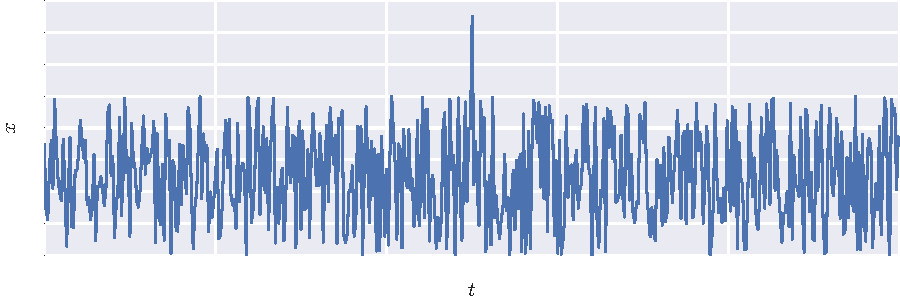
\includegraphics{figs/trivial.pdf}
  \caption{Simple point anomaly}
\end{figure}


\textbf{Context:} Some point anomalies are defined within a context. In Figure \ref{fig:contextanom}, the anomalous point's value is within the range of typical values. But if the cyclic nature of the series were removed, the anomaly is readily detected (`converted' to a simple point anomaly).

\begin{figure}[H]
  \centering
  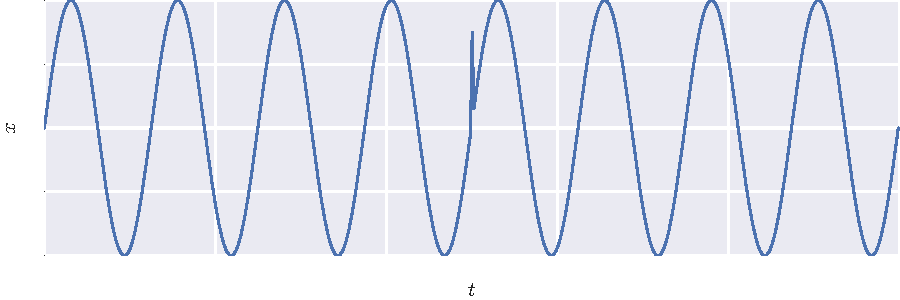
\includegraphics{figs/context.pdf}
  \caption{Anomaly in a periodic context}
  \label{fig:contextanom}
\end{figure}


\subsection{Discord}

Anomalies over subsequences are called discords \cite{Cheboli2010}. In Figure \ref{fig:perdiscordanom}, about two cycles in a periodic time series are unlike the other cycles. The repeated units do not have to be periodic as in Figure \ref{fig:aperdiscordanom}.

\begin{figure}[H]
  \centering
  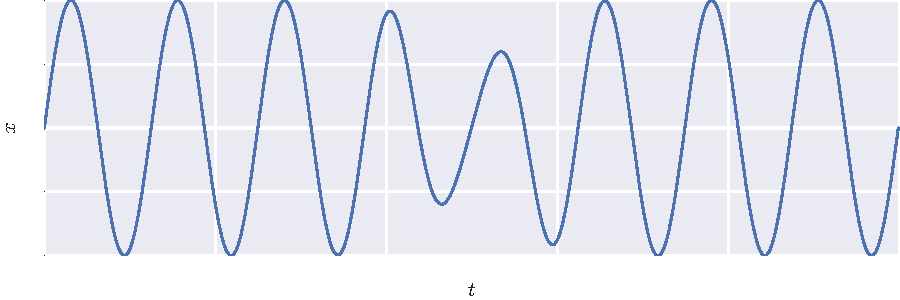
\includegraphics{figs/discord_per.pdf}
  \caption{Discord anomaly in a periodic time series}
  \label{fig:perdiscordanom}
\end{figure}

\begin{figure}[H]
  \centering
  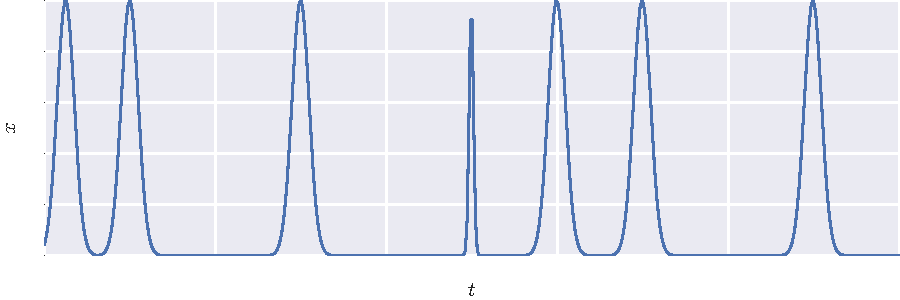
\includegraphics{figs/discord_aper.pdf}
  \caption{Discord anomaly in an aperiodic time series}
  \label{fig:aperdiscordanom}
\end{figure}

\subsection{Multivariate}

Multivariate\footnote{In this text, dimensionality of the time series will refer to the length of the time series as opposed to the number of its variables. Time series anomaly detection literature is inconsistent in the terminology used to refer to these two attributes.} time series add another element of complication for detecting anomalies in them and are not a focus in this work. \cite{Cheboli2010} classifies multivariate time series according to a combination of periodicity and synchronicity: Variables in a time series can be synchronous and periodic, synchronous and aperiodic, asynchronous and periodic, asynchronous and aperiodic. Therefore, any deviation from these properties are anomalies.




\section{Procedure}


In this section, a procedure to find anomalies in time series will be outlined to help answer the questions posed in the introduction of this chapter. The focus will be on issues related to time series as opposed to the general anomaly detection problem. However, there will be a focus on the issues related to solving the general problem of finding anomalies in (an arbitrary) time series as opposed to finding anomalies in a particular application domain. Also, computational issues will not be emphasized.

By examining many detection techniques, a general procedure (Section 2.7 in \cite{Cheboli2010}) can be gleaned:

\begin{enumerate}
\item Compute an anomaly score for an observation (a point or a subsequence in a time series). The anomaly score is a deviation from some `normal' value such as the prediction from a model or similarity to other observations.
\item Aggregate the anomaly scores for many observations.
\item Use the anomaly scores to determine whether an observation can be considered anomalous. For example, an observation could be considered anomalous if its anomaly score exceeds three standard deviations from the mean of the anomaly scores.
\end{enumerate}

At a high level, the procedure is rather straightforward. But, the process of finding what is normal is not. This section is devoted to explaining why finding anomalies in time series is particularly challenging. Addressing the stated problem, given an (single) arbitrary time series, the process of finding normal behavior involves the following steps:
\begin{enumerate}
\item Extract Samples
\item Transform Samples
\item Apply Detection Technique
\end{enumerate}

\subsection{Sample Extraction}
\label{sec:adsample}

Many instances of data are needed to inform what is normal. So, subsequences need to be extracted from a (long) sequence.

Samples can be extracted from a sliding a window over the time series. More precisely, beginning at step $t=0$, sliding a window of width $w$ over a time series $x$ of length $T$ one step at a time produces $p=T-w+1$ windows, $\mathcal{X}=\{W_1,W_2,\ldots,W_p\}$\footnote{In literature, this form corresponds to a time series database \cite{Gupta2013}}.

Now, $\mathcal{X}$ contains all possible subsequences of $\x$ of length $w$ and the value $p$ is typically not much less than $T$. Having many subsequences helps to localize the anomaly; so the window capturing the anomaly will have a higher anomaly score than adjacent windows.

But sometimes it is not desirable for computational reasons to process all subsequences. $p$ can be reduced by introducing a `hop', $h$, that skips $h$ steps when advancing the window from the previous one ($h=1$ gives all possible subsequences).

However, by introducing a large enough hop, anomalies could be missed. Consider the sequence \emph{abc\underline{c}abcabc}. The second \emph{c} is an anomaly. Now inspect the windows generated by various values of $h$ in Table \ref{tbl:hop}. The anomalous \emph{c} is captured in a window when $h$ is 1 or 2 but not when $h$ is 3 or 4. As a general rule, when $h=1$, an anomaly would never be missed. But when $h>1$, there is a chance that anomalies would be missed.

\begin{table}[h]
  \centering
  \begin{tabular}{|c|c|}
    \hline
    hop ($h$) & Ordered Windows \\
    \hline
    \hline
    1 & \emph{abc},
        \emph{bc\underline{c}}, 
        \emph{c\underline{c}a}, 
        \emph{cab},
        \emph{abc}, 
        \emph{bca},
        \emph{cab},
        \emph{abc} \\
    \hline
    2 & \emph{abc},
        \emph{c\underline{c}a},
        \emph{abc},
        \emph{cab} \\
    \hline
    3 & \emph{abc}, 
        \emph{cab},
        \emph{cab} \\
    \hline
    4 & \emph{abc}, 
        \emph{abc} \\
    \hline
  \end{tabular}
  \caption[Point anomalies in sliding windows of various hop sizes]{Point anomalies in sliding windows of width 3 for various hop sizes for the sequence \emph{abc\underline{c}abcabc} are underlined (The \emph{c} in the first \emph{cab} for $h=1$ cannot be considered anomalous because it is not in its context). From \cite{Cheboli2010}.}
  \label{tbl:hop}
\end{table}

\begin{sloppypar}% bc the seq was getting into the margin
Another issue that needs to be considered when working with windows is that the window size must be large enough to capture an anomaly. Consider the sequence \emph{aaabbbccc\underline{c}aaabbbcccaaabbbccc} where the fourth \emph{c} is anomalous. The window width must be at least 4 to capture the fourth \emph{c}. In other words, the window size must be on the order of the anomalous behavior.
\end{sloppypar}

Now given $\mathcal{X}$ for some $w$, the problem may be posed as a multidimensional anomaly detection problem. In this setting, assuming that $\x$ is univariate, samples of $\mathcal{X}$ correspond to $w$ dimensions. However, doing so largely ignores the temporal nature of $\x$. These issues will be discussed within the forthcoming parts of this chapter.

Finally, subsequent steps taken in the anomaly detection process may put restrictions on $h$ and $w$. For example, if the window size is too large, there may not be enough samples to properly apply an anomaly detection technique.

\subsection{Transformation}

Anomalies can be more easily detected if the time series are analyzed in a different representation. Usually these representations are of lower fidelity but capture the essential characteristics of the time series in certain cases. As a general example, a real-valued time series could be or should be discretized into a finite set of symbols or numbers to make use of techniques from bioinformatics. Or, it could be transformed into a different domain such as the frequency domain to make use of techniques from signal processing. As an added benefit, the tranformed time series need less computation given their reduced representation.

More specifically, the Symbolic Aggregate approXimation (SAX) \cite{Lin2007} is an example of time series discretization used to find anomalies in  \cite{Keogh2005}. While the Haar transform represents a transformation to the frequency domain for the same purpose in \cite{Bu2007,fu2006finding}.

However, as a transformation only captures the essential characteristics of a time series, more subtle anomalies could be lost in the transformation process. For example, the anomaly in Figure \ref{fig:contextanom} would be difficult to encode in terms of frequency because it is localized in time while oscillations (representing frequencies) are not.

Another issue to consider is the similarity of the arrangment of time series `points' (like elements of $\mathcal{X}$ in $\mathbb{R}^w$) in the transformed space to that of the original space. Some anomaly detection techniques rely on a certain distribution of points in a space. Suppose an anomaly detection technique works in $\mathbb{R}^w$ by identifying points that are far away from some normal cluster of points. This arrangement should also be present in the transformed space. Anomaly detection techniques that rely on spaces are introduced in Section \ref{sec:adproximity}.

However, a recent empirical study \cite{Wang2013} suggests that, in general, there is little to differentiate between numerous time series representations. Only spectral transformations applied to periodic series showed some advantage but only in certain cases.

\subsection{Detection Technique}

Choosing the anomaly detection technique is the final step in setting up an anomaly detection process. Discussion of detection techniques are discussed as a separate chapter to allow for more development.

\chapter{Detection Technique}
\label{ch:adtechnique}

The application of anomaly detection in a wide variety of domains has led to the development of numerous detection techniques. Each of these applications defines anomalies in a different way;  some  may only be interested in single anomalous points while others are more concerned about anomalous subsquences (discords). Furthermore, techniques are developed drawing on theory from statistics, machine learning, data mining, information theory, and spectral theory.

A highest-level categorization of these techniques could be as follows. The categories are not exhaustive but capture a wide variety of techniques discussed in literature.

\begin{description}

\item[Segmentation] In segmentation-based techniques, the time series is first split into homogeneous segments. Then a finite-state automation is trained to learn transition probabilities between segments. So, a segmented anomalous time series should not have high transition probability \cite{Salvador2005,mahoney2005trajectory,Chan2005}.

\item[Information Theory] Information-theoretic techniques quantify a notion of information content such as entropy. So, a point is considered an anomaly if its removal reduces the information content significantly \cite{Muthukrishnan2004,jagadish1999mining}. That is, anomalous points increase disorder, or require more information to be represented in the sequence.

\item[Proximity] Techniques based on proximity map time series onto a space. It is expected that anomalous time series are `different' because they are far from normal ones.

\item[Model] The difference between the (actual) values of a time series and its predicted values from a model indicate how anomalous they are.
 
\end{description}


Given the variety of techniques applied in different application domains, it is not always possible to use a solution developed for one problem and apply it to another. Finding a general anomaly detection technique is difficult. To the author's knowledge, only one study \cite{Cheboli2010} attempted to compare anomaly detection techniques over a wide variety of data. The study showed, as expected, varying performance of the techniques. A combination of time series characteristics and algorithm settings were sometimes used as explanations for the varying performance. These explanations do not help to objectively determine \emph{a priori} what technique to use and how to adjust any parameters it might use.

It would be difficult to use information theoretic techniques because finding an information theoretic measure sensitive enough to detect a few anomalies is challenging \cite{Chandola2009}. Segmentation-based techniques require that a time series to be made of homogeneous segments. These conditions are deemed too restrictive to be able to solve the general problem. In addition, both are not well-studied. So, they are not further explored here.

This leaves model-based techniques and proximity-based techniques as potential solution categories. Both are widely studied. Furthermore, it is possible to make a theoretical comparison between model-based techniques and proximity-based techniques if they are evaluated as, respectively, generative and discriminative models \cite{Ng2006}. Model-based techniques are usually preferred for anomaly detection \cite{Ngkvist2014} assuming enough training data are available.

Obviously, a good model is needed as well; recurrent neural networks will be introduced in the next chapter. However, proximity-based solutions are explored in this chapter as a benchmark for comparison as they are well-studied and have had numerous successful applications. Also, the hidden Markov model is introduced as an example of model-based solutions in this chapter as another benchmark.


\section{Proximity}
\label{sec:adproximity}

As previously mentioned, proximity-based techniques map time series as points of dimension $w$ in some space using some distance measure. The distance measure is used to evaluate how close a test time series is to others; anomalous time series are those that a far (dissimilar) from those considered normal.

This implies that the time series `points' are arranged in a certain way in the space. In two dimensions, the simplest distribution is portrayed in Figure \ref{fig:simple_dist}. Normal points, $\mathcal{N}_1$, are somewhat clustered. To test whether $p_1$ is an anomaly, it is easy to see, and calculate, that point $p_1$'s nearest neighbor is larger than the nearest neighbor distances of all other points.

\begin{figure}[H]
  \centering
  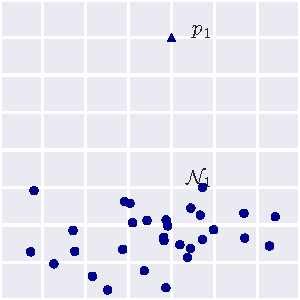
\includegraphics{figs/simple_dist.pdf}
  \caption{Simple anomaly distribution}
  \label{fig:simple_dist}
\end{figure}

Practically, this idealization never occurs. It is not as simple to objectively distinguish $p_1$ and $p_2$ from $\mathcal{N}_1$ and $\mathcal{N}_2$ in the situations depicted in Figure \ref{fig:hard_dist}.

\begin{figure}[H]
  \centering
  \begin{subfigure}[H]{2in}
    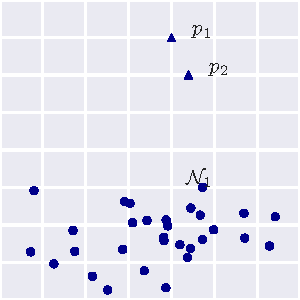
\includegraphics{figs/hard1_dist.pdf}
    \caption{}
    \label{fig:hard1_dist}
  \end{subfigure}
  \begin{subfigure}[H]{2in}
    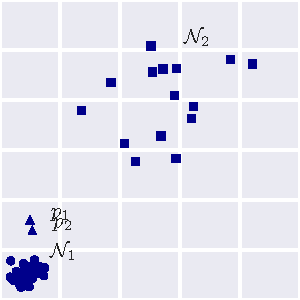
\includegraphics{figs/hard2_dist.pdf}
    \caption{}
    \label{fig:hard2_dist}
  \end{subfigure}
  \caption{Complex anomaly distribution}
  \label{fig:hard_dist}
\end{figure}


\subsection{Effects on Point Distribution}

Having complex distributions is the purview of anomaly detection in general and not a problem particular to time series data. However, issues influenced by the temporal nature of the data will be the focus of this subsection.

\subsubsection{Distance Measure}%

The choice of distance measure is crucial for anomaly detection because it captures some intuitive notion of similarity between a pair of time series. It is possible to use the `ordinary' Eucilidean distance \cite{Keogh2002} but it does not always capture the desired similarity between a pair of time series. The comparison between time series should be invariant to the following factors:

\begin{description}

\item[Length]  \hfill \\
%
Sometimes it is desirable to be able to compare sequences of different lengths. Compare the sequence, \emph{ababababab}, to a shorter one, \emph{abababa}. There is reason to believe that both are at least highly similar.

\item[Skew] \hfill \\
%
Consider the sequence \emph{abaababaaabaabab} and \emph{aaababaababaabab} where occurances of \emph{b} are padded by an unpredictable number of \emph{a}'s. The sequences can be considered similar even if they are not strictly periodic.

Dynamic Time Warping (DTW) \cite{Keogh2002} is capable of identifying similarity in such scenarios by `warping' the sequences to minimize dissimilarity (DTW is also capable of comparing sequences of different lengths).

\item[Translation] \hfill \\
%
Typically, sequences that are shifted in time are considered similar. For example, \emph{abababab} is similar to \emph{babababa}. Despite the sophistication of DTW, a warping transformation would not make these two sequences similar.  Cross-correlation is a similarity measure that can handle translations \cite{Protopapas2005}.

\item[Amplitude] \hfill \\
%
Sometimes it is desirable to ignore differences in amplitude if two time series are otherwise similar. Distance measures are usually sensitive to differences in amplitude unless the time series are normalized \cite{Keogh2002}. 

\end{description}

So simple measures, like the Euclidean distance, are not able to accommodate these factors. However, recently, in a comprehensive study of similarity measures, \cite{Wang2013} finds that, in large data sets, the clustering accuracy of `elastic' measures, such as DTW, converges with that of the Euclidean distance. Nonetheless, the advantage of using DTW, as well as other elastic measures, is maintained for smaller data sets.

Furthermore, in addition to addressing the previously mentioned factors, the distance measure must be compatible with the time series representation \cite{Chakrabarti2002}. So, for example, if a symbolic representation is used, then the distance measure must be appropriate for symbolic data.


\subsubsection{Window Width}

Section \ref{sec:adsample} introduced the use of sliding windows to extract samples of some width\footnote{Window `size' or `length' might also be used to refer to window width}, $w$. Here, the effect of the choice of $w$ will be explained when combined with a distance measure.

Also in Section \ref{sec:adsample}, it was mentioned that $w$ should be, at least, on the order of the length of the expected anomaly. But when $w$ is too large the distance measure becomes less effective at measuring similarity because the proportion of the anomalous subsequence becomes small compared to $w$. Furthermore, pairs of points become more equidistant in high-dimensional space \cite{Hinneburg2000,Beyer1999} which makes distinguishing between time series difficult (though this could be mitigated by using a dimension-reducing transformation \cite{Keogh2001}).


\subsubsection{Sliding Windows}
\label{sec:sliding}

The mere action of extracting samples with a \emph{sliding} window (with a small $h$, in contrast to non-overlapping windows) can have a profound effect on the distribution of the samples in the space. The effects challenge assumptions about the organization of (sliding window) points for the task of anomaly detection.

\cite{Keogh2005} demonstrates that anomalous anomalous points are not necessarily located in sparse space. Conversely, repeated patterns are not necessarily located in dense space \cite{kitaguchi2004extracting,Chiu2003,Bentley1997}.

Furthermore, in a paper challenging the status quo, \cite{Keogh2004} makes the bold claim that clustering of time series with sliding windows is meaningless. It found no similarity between clusters found with a sliding window ($h<<w$) and clusters found when the windows did not overlap ($h>w$) which invalidated the results of previously published papers per its argument. However, some constraints were identified that may allow some data sets to be clustered. But a decade later, the issue of clustering subsequences of time series is unresolved \cite{Zolhavarieh2014}.

These findings place restrictions on selecting a proximity-based anomaly detection algorithm.


\subsection{Data Classification}

In the following subsections, data classification techniques (that facilitate anomaly detection) will be discussed. The techniques are not particular to time series data. However, finding anomalous windows of time series data is referred to as `discord detection' in literature.

\subsubsection{Local versus Global Techniques}

First it is instructive make a general note about how they work regardless of how they are classified.

Proximity-based anomaly detection techniques can use a global context (of all) data points or a local context to test whether a point is an anomaly. Going back to Figure \ref{fig:simple_dist}, it was mentioned that it is trivial to find the anomalous point using all data points. However, in \ref{fig:hard2_dist}, it is not trivial to distinguish $p_11$ and $p_2$ as anomalous in this global view due to their proximity to $\mathcal{N}_1$. An anomaly detection approach that considers the (local) neighborhood of points $p_1$ and $p_2$ must be used.

\subsection{Nearest-Neighbor}

Nearest-neighbor techniques assume that normal points are in dense neighborhoods while anomalies are far from them.

In the beginning of Section \ref{sec:adproximity}, it was noted how simple it is to determine that point $p_1$ in Figure \ref{fig:simple_dist} is anomalous. However, given the discussion about sliding windows in Section \ref{sec:sliding}, it is not as straightforward when dealing with data points generated from sliding windows.

The problem comes from adjacent windows being close to each other in space. Consider the windows of width equal to 3 for the sequence \emph{abcabcXXXabcababc} \cite{Keogh2005} in Figure \ref{tbl:selfmatch}. Obviously, the subsequence \emph{XXX} stands out as the most anomalous after \emph{bab}. But \emph{XXX} has the nearest matches \emph{cXX} and \emph{XXa} one step away as can be seen in the subsequences generated by advancing a window on every step ($h=1$). This makes the subsequence \emph{bab} as more anomalous because is it different by two symbols from its nearest match \emph{aba}. In contrast, when examining windows with no overlap ($h=3$), \emph{XXX} is far from all other subsequences.

\begin{table}[h]
  \centering
  \begin{tabular}{|c||c|}
    \hline
    $h=1$ & $h=3$ \\
    \hline
    \hline
    \emph{abc} & \emph{abc} \\
    \emph{bca} & \\
    \emph{cab} & \\
    \hline
    \emph{abc} & \emph{abc} \\
    \emph{bcX} & \\
    \emph{cXX} & \\
    \hline
    \emph{XXX} & \emph{XXX} \\
    \emph{XXa} & \\
    \emph{Xab} & \\
    \hline
    \emph{abc} & \emph{abc} \\
    \emph{bca} & \\
    \emph{cab} & \\
    \hline
    \emph{aba} & \emph{aba} \\ 
    \emph{bab} & \\
    \emph{abc} & \\
    \hline
  \end{tabular}
  \caption[Neighbors of sliding windows]{Neighbors of sliding windows of sequence \emph{abcabcXXXabcababc}}
  \label{tbl:selfmatch}
\end{table}

However, it is still possible to use overlapping windows to find subsequences like \emph{XXX}. The solution proposed by  \cite{Keogh2005} is to use non-self matches. So when when calculating distances (similarity) to neighbors of \emph{XXX}, only those that are at least one window width away are considered. In this calculation, \emph{XXX} would not have any neighbors with the symbol \emph{X}.

Furthermore, the solution in \cite{Keogh2005} improves upon the brute force discord search by employing a heuristic called HOT SAX: Heuristically Ordered Time series using Symbolic Aggregate approXimation. But the time series is discretized as part of its process.

If the issues with sliding windows can be mitigated, it is possible to use anomaly detection techniques that are not specific to time series. Nearest-neighbor techniques can use either the $k$th nearest neighbor (kNN) distance or the relative density of a region around a point in the calculation of its anomaly score.

For example, the kNN distance can be used to identify that $p_1$ and $p_2$ are anomalies in Figure \ref{fig:hard1_dist}. By choosing, say, $k=4$, the fourth nearest neighbor of points $p_1$ and $p_2$ would be a point in \emph{far} away in $\mathcal{N}_1$. While the fourth nearest neighbor for a point in $\mathcal{N}_1$ is always a \emph{nearby} point within $\mathcal{N}_1$. 

The HOT SAX technique was introduced as, what is essentially, a $k=1$ kNN technique. But it can be generalized to an arbitrary $k$ \cite{Keogh2007,Yankov2008}.

However, kNN techniques cannot deal with data sets of varying density. Going back to Figure \ref{fig:hard1_dist}, if $\mathcal{N}_1$ were denser, so that distances between points in $\mathcal{N}_1$ were less than the distance between $p_1$ and $p_2$, then $k$ can only equal to 2. Generally, $k$ needs to be equal to the number of anomalous points as long as the clustering of $\mathcal{N}_1$ is denser than the clustering of $p_k$. But since some distances between between pairs of points in $\mathcal{N}_1$ are similar to the distance between $p_1$ and $p_2$, $k$ has to be greater than 2. Furthermore, a further complication can be considered if another normal set of points, $\mathcal{N}_2$, is included as in Figure \ref{fig:hard2_dist}. Here, it is not simple to find a value of $k$ that would not distinguish $p_1$ and $p_2$ due to the varying densities in $\mathcal{N}_1$ and $\mathcal{N}_2$.

But by using local density information, techniques based on the relative density of a point's region can mitigate this problem. For example, \cite{Breunig1999} defines a Local Outlier Factor (LOF) for a point that is the ratio of the average local density of its $k$ nearest neighbors to the local density of the point itself. The local density is defined as $k$ divided by the volume of the smallest hypersphere that contains $k$ nearest neighbors. In other words, a point is likely to be an anomaly if its neighbors are in dense regions while it is in a less dense region. Applied to Figure \ref{fig:hard2_dist}, the LOF for points in $\mathcal{N}_1$ and $\mathcal{N}_2$ is similar. But for points $p_1$ and $p_2$, if two nearest neighbors are considered, the second nearest neighbor would be the closest point in $\mathcal{N}_1$ where its local density is high compared to the local density of $p_1$ and $p_2$ resulting in a LOF that is higher than the LOF of points in $\mathcal{N}_1$ and $\mathcal{N}_2$. This is true for any $k>2$.

In any case, nearest neighbor techniques rely on normal points being in denser regions. But given the discussion about the effect of sliding windows in Section \ref{sec:sliding}, it is not clear how these techniques would be generally applicable to time series data.

\cite{Chandola2009} provides a more thorough treatment for general data types.


\subsection{Clustering}

Clustering algorithms are used to group similar points. Typically they are not used to find anomalies but they can be adapted to do so if some assumptions are made.

One assumption that could be made is that normal points belong to clusters while anomalies do not. This requires algorithms that do not force all points to belong to a cluster such as the well-known DBSCAN \cite{Ester1996} algorithm where deviant points are considered noise. Still, such algorithms are optimized to find clusters. So anomalous points could incorrectly be included in a cluster.

Another assumption that could be made resembles nearest neighbor techniques; anomalous points are far from their nearest cluster's centroid while normal points are not. Any clustering algorithm could be used such as K-means \cite{Munz2007}. However, this assumption would misclassify anomalous points that form clusters themselves.

A third assumption could be that normal points are in large and dense clusters while anomalous points are in small and sparse clusters. In similar fashion to LOF, described previously, a Cluster-Based Local Outlier Factor (CBLOF) was introduced in \cite{He2003}. But, again, given the discussion about sliding windows in \ref{sec:sliding}, it is not clear how these techniques would be generally applicable to time series data.

\cite{Chandola2009} provides a more thorough treatment for general data types.


\section{Models}

Instead of comparing a point to other points, like in proximity-based solutions, a point can be compared to what is expected from a model. 

For example, Hidden Markov Models (HMM) are advanced sequence modelers and therefore can be used for anomaly detection \cite{Zhang2003,Qiao2002,qiao2002anomaly,Florez-Larrahondo2005}. To use in anomaly detection, first, a HMM maximizes the probability of a set of training data. Then the probability of a test instance is calculated for comparison. But the comparison is only meaningful if the training data can be modeled by the hidden Markovian process.

Moreover, sequence modelers typically require training examples of fixed length which restricts the `memory' of the model.


\section{Conclusions} 

Some general comments can be made regarding the strengths and weaknesses of general anomaly detection techniques such as those in Section 11 of \cite{Chandola2009} for example. However this does not provide any rigorous and objective evaluation. An objective evaluation is needed in order to select the most appropriate algorithm for the problem \emph{a prioi}. In \cite{Cheboli2010} and \cite{Chandola2008} some qualitative explanation is given for the performance of several time series anomaly detection techniques over various data sets. Still, this does not objectively determine why one technique performs better.

Exceptionally however, \cite{Schubert2014} outlines a theoretical framework for local outlier detection in which different methods are assessed in this common view. Perhaps surprisingly, different methods were found to be similar including those used in quite different application domains. Similarly, \cite{knorr1997unified} unify anomalies identified based on some distance with anomalies identified based on a statistical model.

For the techniques discussed in this text, a number of issues specific to time series data (as well as issues not specific to time series data) combine in the process of using a proximity-based (discriminative) technique for anomaly discussion. The choices of similarity measure, sliding window width, sliding window hop, and classification technique must be compatible. Furthermore, defining a region for every normal behavior is difficult to begin with.

So the case is made for generative model-based solutions due to these complications. Models provide a better summary of data which gives it a robustness that is preferred for the task of anomaly detection \cite{Ngkvist2014}. Given this preference, proximity-based methods would only be preferable if modeling the time series is difficult (disregarding computational issues).

This work attempts to find anomalies in an arbitrary time series. So, an anomaly detection process is sought that:
\begin{itemize}
\item models arbitrary time series,
\item minimizes the effects of window width,
\item and requires as few parameters as possible.
\end{itemize}

This guides the discussion in the next two chapters. The next chapter shows how recurrent neural networks are general sequence modelers. In the following chapter, a procedure is outlined that addresses windows width and model parameters.



%%% Local Variables:
%%% mode: latex
%%% TeX-master: "thesis"
%%% End: